\begin{appendices}

\section{Analytical Derivation of the Local Gradient}
\label{appendix:derivation}
In the following we derive an expression for the gradient that is specific to our system.
Since the loss function depends on the field only through the two detector scores, the chain rule gives
\begin{align}
    \frac{\mathrm{d}\mathcal{L}(s_1, s_7)}{\mathrm{d}p}
    =\frac{\partial \mathcal{L}}{\partial s_1}\frac{\mathrm{d}s_1}{\mathrm{d}p}
    +\frac{\partial \mathcal{L}}{\partial s_7}\frac{\mathrm{d}s_7}{\mathrm{d}p}.
    \label{eq:dL/dp-chain}
\end{align}
The specific choice of loss function enters only through the two prefactors $\partial\mathcal{L}/\partial s_c$. 
Both are real-valued, since $\mathcal{L}$ is real by construction. Everything that follows is independent of that choice.

The remaining derivatives $\mathrm{d}s_c/\mathrm{d}p$ describe how the detected intensities respond to a change of $p$. 
We write the score of channel $n$ as $s_n = E_{\mathrm{out},n}(p)\,E_{\mathrm{out},n}^{*}(p)$ and treat field and conjugate field as independent variables. 
This yields
\begin{align}
    \frac{\mathrm{d}s_n}{\mathrm{d}p}
    =\frac{\partial s_n}{\partial E_{\mathrm{out},n}}
     \frac{\mathrm{d}E_{\mathrm{out},n}}{\mathrm{d}p}
    +\frac{\partial s_n}{\partial E_{\mathrm{out},n}^{*}}
     \frac{\mathrm{d}E_{\mathrm{out},n}^{*}}{\mathrm{d}p}
    =E_{\mathrm{out},n}^{*}\frac{\mathrm{d}E_{\mathrm{out},n}}{\mathrm{d}p}
    +E_{\mathrm{out},n}\frac{\mathrm{d}E_{\mathrm{out},n}^{*}}{\mathrm{d}p}.
    \label{eq:ds/dp}
\end{align}
Because $p$ is a real-valued phase, differentiation commutes with complex conjugation, $\mathrm{d}E^{*}/\mathrm{d}p=(\mathrm{d}E/\mathrm{d}p)^{*}$. 
The two terms in \eqref{eq:ds/dp} are therefore complex conjugates of each other and their sum reduces to twice the real part of either one.
Inserting this into \eqref{eq:dL/dp-chain} and moving the real prefactors inside the real part, we obtain
\begin{align}
    \frac{\mathrm{d}\mathcal{L}}{\mathrm{d}p}
    =2\,\Re\left\{
        \frac{\partial \mathcal{L}}{\partial s_1}\,
        E_{\mathrm{out},d_1}^{*}
        \frac{\mathrm{d}E_{\mathrm{out},d_1}}{\mathrm{d}p}
       +\frac{\partial \mathcal{L}}{\partial s_7}\,
        E_{\mathrm{out},d_7}^{*}
        \frac{\mathrm{d}E_{\mathrm{out},d_7}}{\mathrm{d}p}
    \right\}.
    \label{eq:dL/dp-realpart}
\end{align}

We now define the error field $\boldsymbol{\Gamma}\in\mathbb{C}^{N}$. 
It quantifies the sensitivity of the loss to a perturbation of the complex field amplitude in each output channel,
\begin{align}
    \Gamma_{n} \equiv
    \frac{\partial\mathcal{L}}{\partial E_{\mathrm{out},n}^{*}}
    = \begin{cases}
        \dfrac{\partial \mathcal{L}}{\partial s_c}\,E_{\mathrm{out},n},
          & n=d_c,\quad c\in\{1,7\},\\[2ex]
        0, & \text{otherwise,}
      \end{cases}
    \label{eq:gamma}
\end{align}
so that \eqref{eq:dL/dp-realpart} takes the compact form
\begin{align}
    \frac{\mathrm{d}\mathcal{L}}{\mathrm{d}p}
    = 2\,\Re\left\{
        \mathbf{\Gamma}^{\dagger}
        \frac{\mathrm{d}\mathbf{E}_{\mathrm{out}}}{\mathrm{d}p}
      \right\}.
    \label{eq:dL/dp-compact}
\end{align}
The benefit of the \gls{avm} already becomes visible in \eqref{eq:gamma}. 
The error field does not depend on $p$, so the same $\boldsymbol{\Gamma}$ serves every tunable phase in the mesh.
%Feldableitung nach p berechnen
\begin{figure}[H]
    \centering
    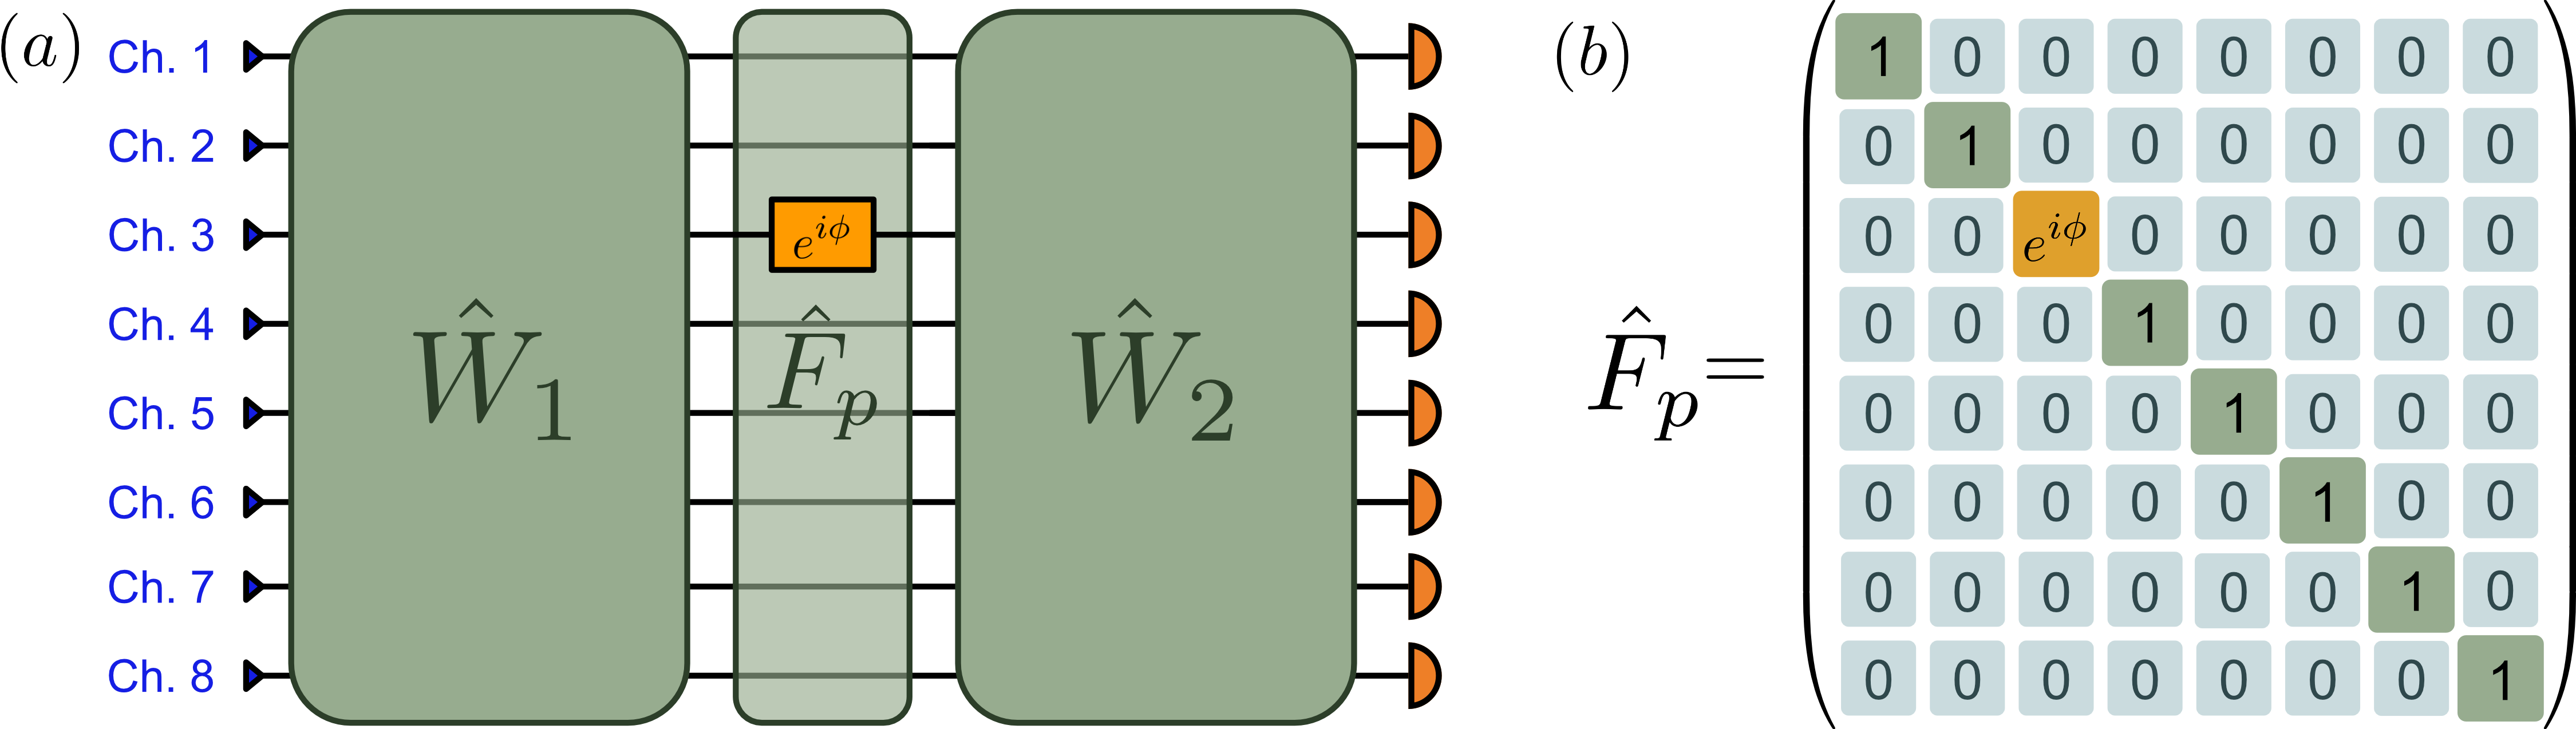
\includegraphics[width=1\linewidth]{images/BlockZerlegungver3.png}
    \caption{(a) Partition of the transfer matrix $\hat{W}$ of an eight-channel \gls{mzi} mesh into a preceding mesh $\hat{W}_1$, an isolated layer $\hat{F}_p$ containing only the phase shifter $p$, and a subsequent mesh
    $\hat{W}_2$. 
    (b) Transfer matrix of the isolated layer $\hat{F}_p$, here for a phase shift acting on channel $q=3$.}
    \label{fig:SplitMesh}
\end{figure}

It remains to evaluate the field derivative 
$\mathrm{d}\mathbf{E}_{\mathrm{out}}/\mathrm{d}p$.
For this we isolate the position in the mesh at which $p$ acts. 
Splitting off this artificial layer $\hat{F}_p$ leaves a preceding mesh $\hat{W}_1$ and a subsequent mesh $\hat{W}_2$, as shown in Figure~\ref{fig:SplitMesh},
\begin{align}
    \hat{W} = \hat{W}_{2}\,\hat{F}_{p}\,\hat{W}_{1},
    \qquad
    \bigl(\hat{F}_{p}\bigr)_{kk} =
    \begin{cases}
        e^{ip}, & k=q,\\
        1,      & k\neq q,
    \end{cases}
    \label{eq:split}
\end{align}
where $q$ denotes the channel on which the phase shifter acts. 
Note that $\hat{F}_p$ is not a physical layer of the mesh. 
Each \gls{mzi} contains two phase shifters, so the cut generally runs through a single \gls{mzi}: 
its first beam splitter belongs to $\hat{W}_1$, while the remaining components belong to $\hat{W}_2$.

Differentiating \eqref{eq:split} affects only the $q$-th diagonal entry,
\begin{align*}
    \frac{\mathrm{d}\hat{F}_{p}}{\mathrm{d}p}
    = i\,e^{ip}\,\mathbf{e}_{q}\mathbf{e}_{q}^{\top},
    \quad \text{with}\
    \mathbf{e}_{q}\in\mathbb{R}^{N},\quad
    \bigl(\mathbf{e}_{q}\bigr)_{k}=\delta_{qk},
    %\label{eq:dFdp}
\end{align*}
Since $\hat{W}_1$ and $\hat{W}_2$ are independent of $p$, they act as constants.
The unit vectors $\mathbf{e}_q$ form an outer product that projects onto the single channel $q$,
\begin{align}
    \frac{\mathrm{d}\mathbf{E}_{\mathrm{out}}}{\mathrm{d}p}
    = \hat{W}_{2}\,\frac{\mathrm{d}\hat{F}_{p}}{\mathrm{d}p}\,
      \hat{W}_{1}\mathbf{E}_{0}
    = i\,e^{i p}\;
      \bigl(\hat{W}_{2}\mathbf{e}_{q}\bigr)
      \underbrace{\bigl(\mathbf{e}_{q}^{\top}\hat{W}_{1}\mathbf{E}_{0}\bigr)}
      _{\textstyle \equiv\, A^{\text{before}}_{p}}.
    \label{eq:dEdp}
\end{align}
Grouping the terms this way isolates a scalar. 
The second bracket is the complex field amplitude $A_p^{\text{before}}$ on channel $q$, immediately in front of the phase shifter. 
It is a quantity that the forward pass produces anyway, and on a physical chip its intensity is accessible through non-invasive on-chip monitors \cite{morichettiNonInvasiveOnChipLight2014}.

Inserting \eqref{eq:dEdp} into \eqref{eq:dL/dp-compact} gives a scalar product with $\boldsymbol{\Gamma}$. 
For a scalar, Hermitian conjugation reduces to complex conjugation, which lets us move $\hat{W}_2$ onto the error field,
\begin{align*}
    \boldsymbol{\Gamma}^{\dagger}\hat{W}_{2}\mathbf{e}_{q}
    = \bigl(\boldsymbol{\Gamma}^{*}\bigr)^{\top}\hat{W}_{2}\mathbf{e}_{q}
    = \mathbf{e}_{q}^{\top}\hat{W}_{2}^{\top}\boldsymbol{\Gamma}^{*}
    = \bigl(\hat{W}_{2}^{\top}\boldsymbol{\Gamma}^{*}\bigr)_{q}.
    %\label{eq:transposestep}
\end{align*}
The transpose $\hat{W}_2^{\top}$ describes propagation from the output ports back to the position of $p$. 
This identification rests on reciprocity of the lossless mesh. 
The conjugated error field $\mathbf{\Gamma}^{*}$ is the source injected at the detectors. 
We define its $q$-th component as the adjoint field amplitude,
\begin{align*}
    A_p^{\mathrm{adj}} \equiv
    \bigl(\hat{W}_{2}^{\top}\mathbf{\Gamma}^{*}\bigr)_{q}.
    %\label{eq:core-Aadj}
\end{align*}
Both $A_p^{\text{before}}$ and $A_p^{\mathrm{adj}}$ are amplitudes taken in front of the phase shifter, each with respect to its own direction of propagation. 
Absorbing the phase factor into the forward amplitude, $A_p \equiv e^{ip}A_p^{\text{before}}$, describes the field directly after the component. 
With $\Re\{i\,z\}=-\Im\{z\}$ we arrive at 
\begin{align}
    \frac{\mathrm{d}\mathcal{L}}{\mathrm{d}p}
    = 2\,\Re\left\{ i\,A_p\,A_p^{\mathrm{adj}} \right\}
    = -2\,\Im\left\{ A_p\,A_p^{\mathrm{adj}} \right\}
    \label{eq:final}
\end{align}
which reproduces the result of \cite{hughesTrainingPhotonicNeural2018}, up to
the factor of two absorbed into their definition of the error field.

Equation \eqref{eq:final} is the result we set out to obtain. 
The gradient with respect to $p$ follows from two field amplitudes at a single location, taken once for the forward field $\mathbf{E}_0$ and once for the backward-propagating error field. 
Both fields traverse the entire mesh in a single pass. 
The cost of a complete gradient evaluation is therefore independent of the number of trainable phases, which is what makes the approach attractive for large meshes.
 
On physical hardware one further step would be required. Photo detectors respond to intensity, so the complex amplitudes in \eqref{eq:final} are not directly accessible.
\citeauthor{hughesTrainingPhotonicNeural2018} address this with the time-reversal interference method, which rests on three principles~\cite{hughesTrainingPhotonicNeural2018}. 
Reciprocity of the lossless mesh makes the backward pass a physically realizable propagation. 
Complex conjugation in the frequency domain corresponds to time reversal, which turns the counter-propagating adjoint field into a co-propagating one. 
Interfering it with the forward field then produces an intensity pattern whose cross term is the required overlap, isolated by subtracting the separately measured constant terms:
\begin{align*}
    I_p = \bigl|A_p + (A_p^{\mathrm{adj}})^{*}\bigr|^{2}
        = |A_p|^{2} + |A_p^{\mathrm{adj}}|^{2}
          + 2\,\Re\left\{A_p\,A_p^{\mathrm{adj}}\right\}.
    %\label{eq:interference}
\end{align*}
The present work focuses on the training method rather than on a full simulation of the physical system. 
We therefore read the field amplitudes $A_p$ and $A_p^{\mathrm{adj}}$ directly from the simulated forward and backward passes, which yields the same gradient \eqref{eq:final} without modeling the measurement protocol.

\section{Additional figures}
\label{appendix:graph}

\subsection{Learning rate analysis}
\label{appendix:graph-learningrate}
\begin{figure}[H]
    \centering
    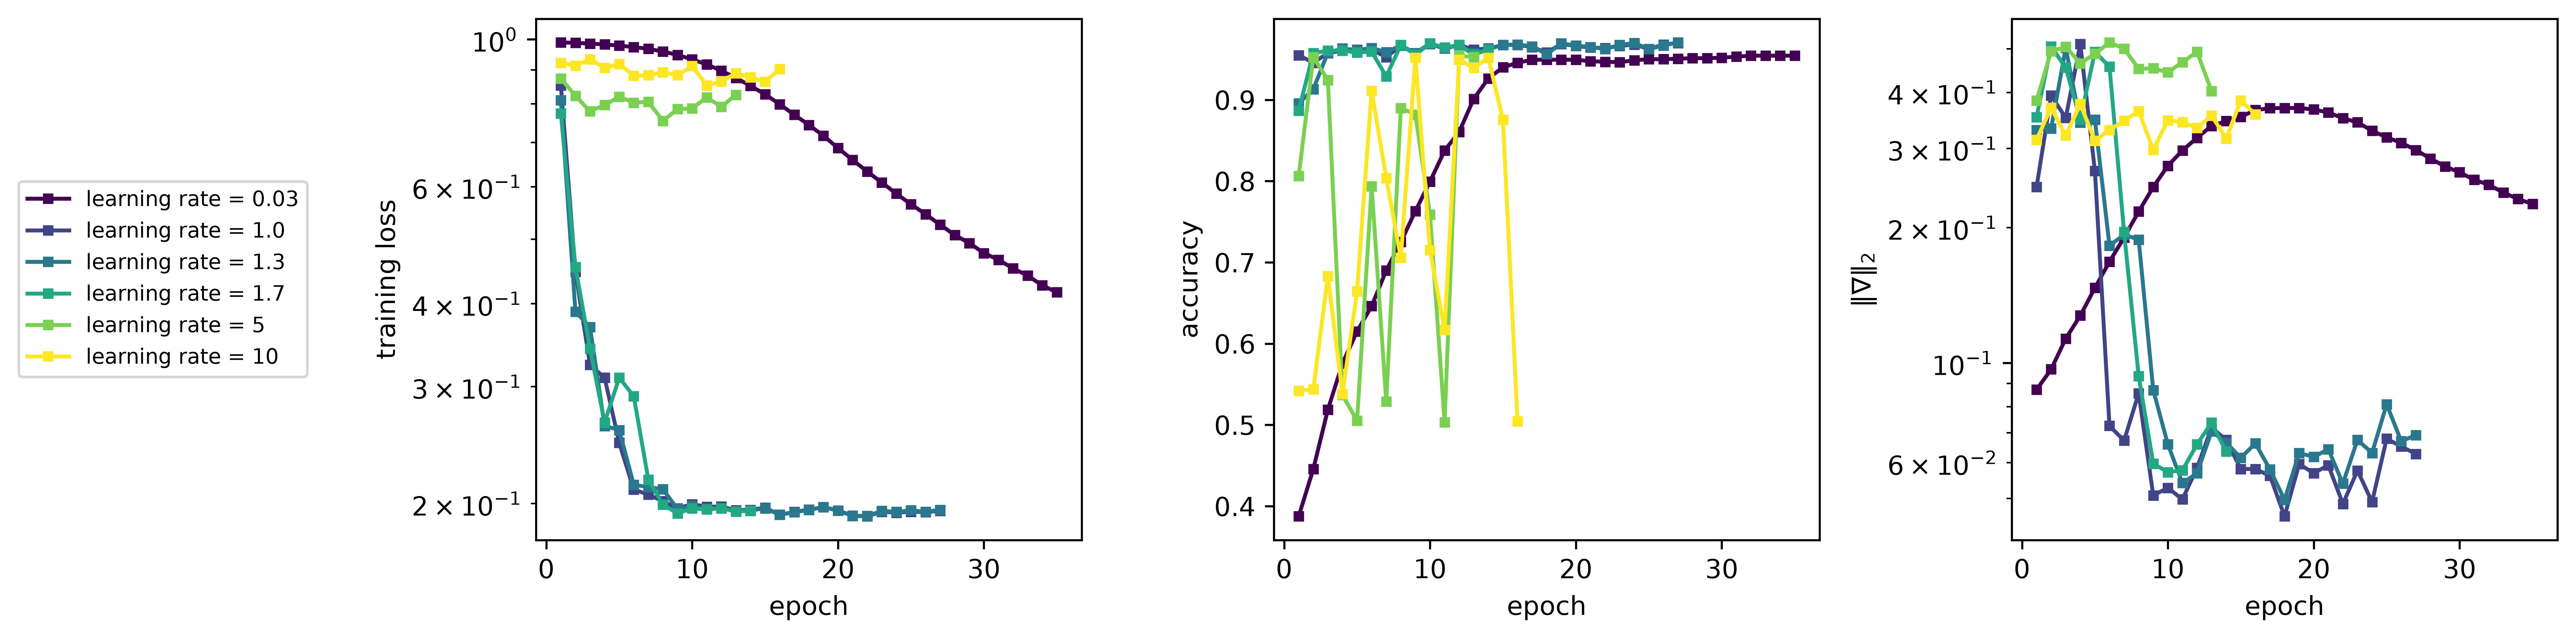
\includegraphics[width=1\linewidth]{evaluation/learning_rate/256_plot_training_epoch.png}
    \caption{Training loss, training accuracy and normalized gradient for different learning rates for a batch size of 256.}
    \label{fig:learning_rate_big_batch_sweep}
\end{figure}

\begin{figure}[H]
    \centering
    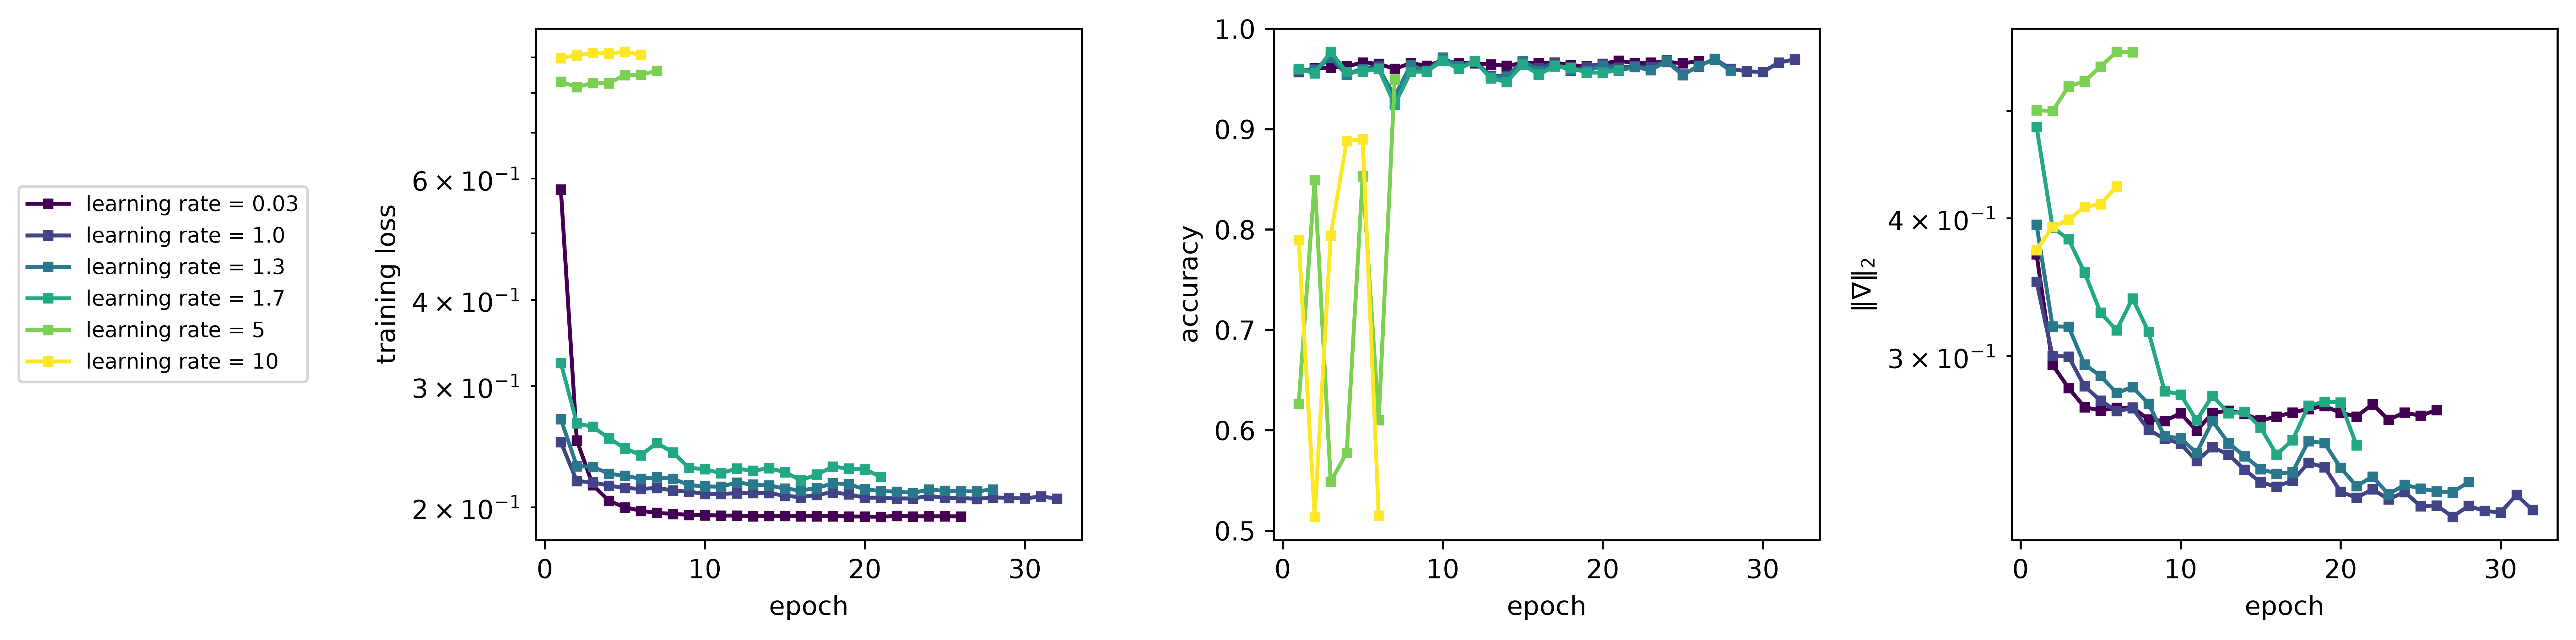
\includegraphics[width=1\linewidth]{evaluation/learning_rate/4_plot_training_epoch.png}
    \caption{Training loss, training accuracy and normalized gradient for different learning rates for a batch size of 4.}
    \label{fig:learning_rate_small_batch_sweep}
\end{figure}

\subsection{Side length analysis (down-sampling)}
\label{appendix:graph-m}
\begin{figure}[H]
    \centering
    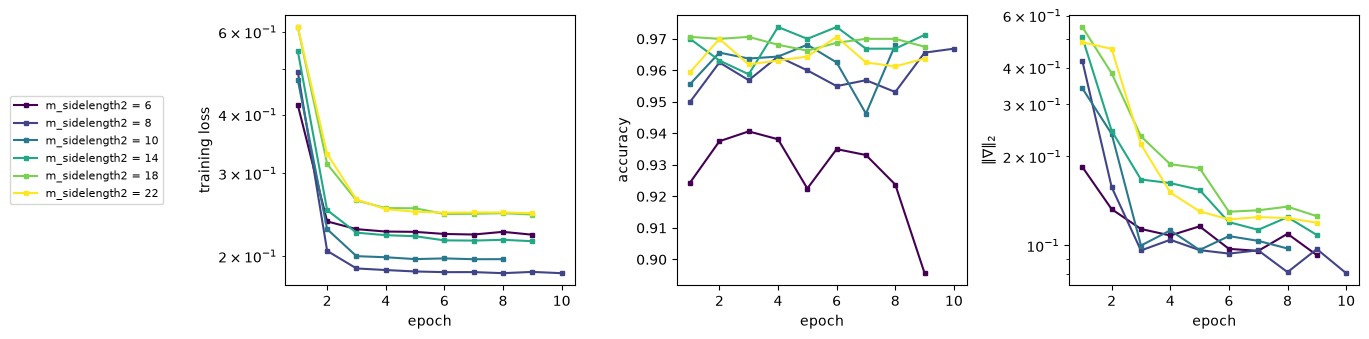
\includegraphics[width=1\linewidth]{evaluation/m_sidelength/plot_training_epoch.png}
    \caption{Training loss, training accuracy and normalized gradient plotted over the epochs for different side lengths of the down-sampled MNIST images.}
    \label{fig:m_sidelength_sweep_epoch}
\end{figure}

\begin{figure}[H]
    \centering
    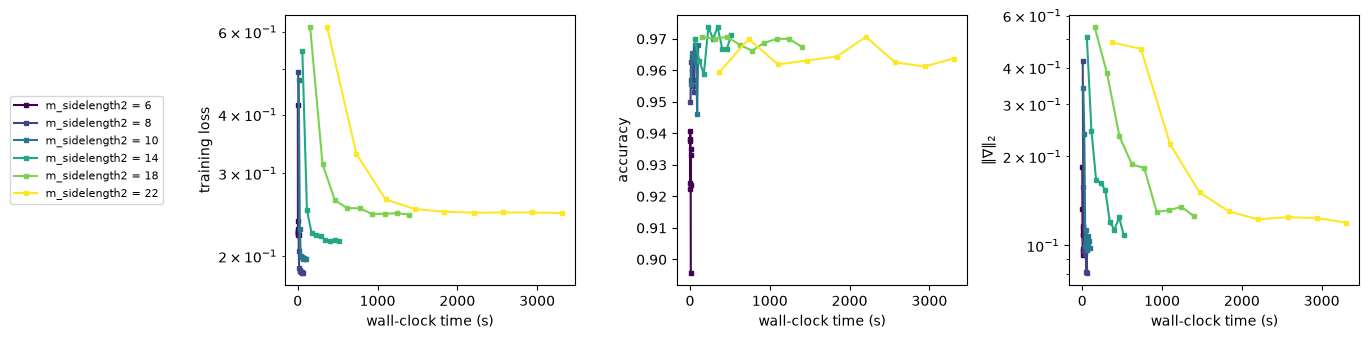
\includegraphics[width=1\linewidth]{evaluation/m_sidelength/plot_training_time.png}
    \caption{Training loss, training accuracy and normalized gradient plotted over the wall-clock time for different side lengths of the down-sampled MNIST images.}
    \label{fig:m_sidelength_sweep_time}
\end{figure}


\subsection{Batch size analysis}
\label{appendix:graph-batchsize}
\begin{figure}[H]
    \centering
    
\includegraphics[width=1\linewidth]{evaluation/batch_size/plot_training_epoch.png}
    \caption{Batch loss, training loss, training accuracy and normalized gradient plotted over the epochs for different batch sizes.}
    \label{fig:batch_size_sweep_epoch}
\end{figure}

\begin{figure}[H]
    \centering
    
\includegraphics[width=1\linewidth]{evaluation/batch_size/plot_training_time.png}
    \caption{Batch loss, training loss, training accuracy and normalized gradient plotted over the wall-clock time for different batch sizes.}
    \label{fig:batch_size_sweep_time}
\end{figure}

\subsection{Hyperparameter theta\_enc (in phase encoding)}
\label{appendix:graph-thetaphase}
\begin{figure}[H]
    \centering
    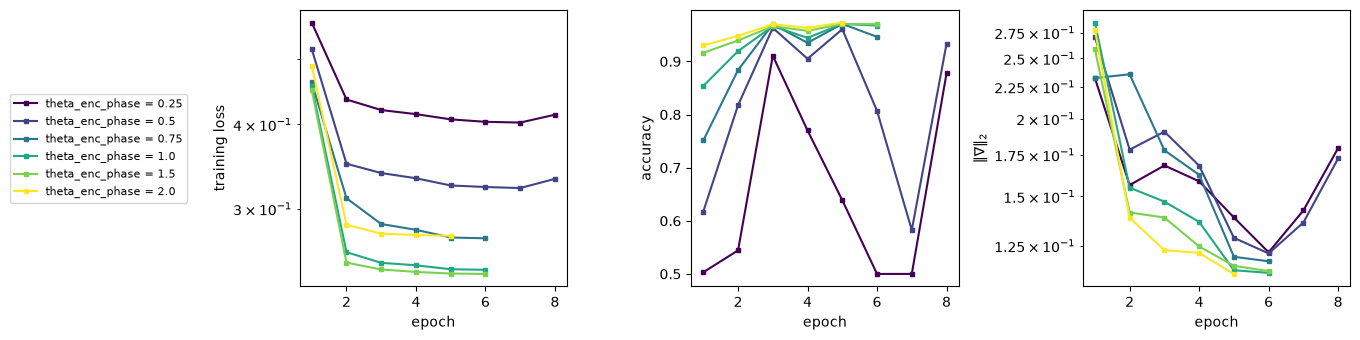
\includegraphics[width=1\linewidth]{evaluation/phase_encoding/output.png}
    \caption{Training loss, training accuracy and normalized gradient plotted over the epochs for different values of \code{theta\_enc} in phase encoding.}
    \label{fig:phase_enc_theta_sweep}
\end{figure}

\subsection{Architecture comparison}
\begin{figure}[H]
    \centering
    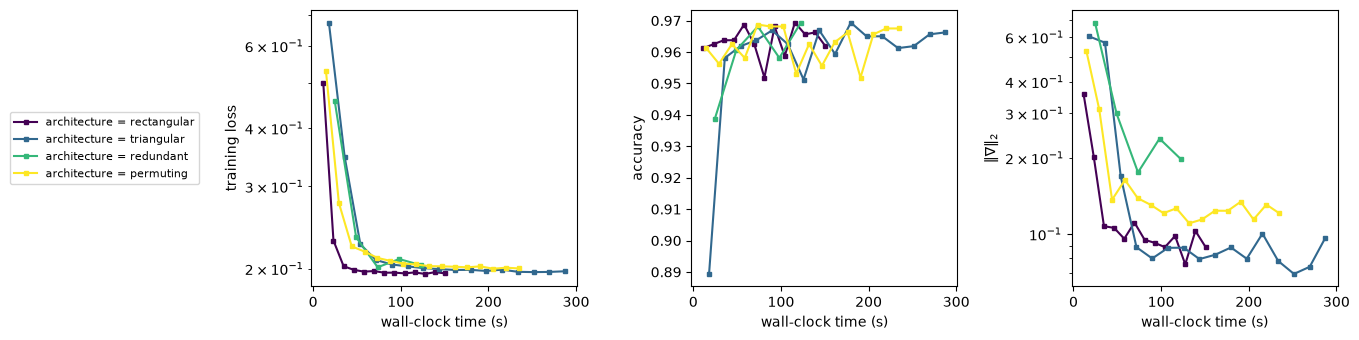
\includegraphics[width=1\linewidth]{evaluation/architecture/output.png}
    \caption{Training loss, training accuracy and normalized gradient for four different architectures of the \gls{mzi} mesh.}
    \label{fig:architecture_sweep}
\end{figure}

\end{appendices}